\section{What pressure disintegration can and cannot detect}\label{sec:disintegration}

A natural thermodynamic test of a strict extension is to disintegrate a reference law over the completion objects and compare the conditional growth rates. This section makes that test precise. It then shows that the outcome is decided by the reference law, not by the extension: on the same shell, with the same potential and the same two completion objects, one admissible law gives a zero gap and another gives a positive one.

\subsection{Reference laws and the weighted gap}

A \emph{reference law} is a probability measure $\Pp$ on states of~$\Sh$, each of which carries its own future. Under $\Pp$ the completion object $\Gamma$ is a random variable. We consider laws for which $\Gamma$ takes finitely many values $\gamma_1,\dots,\gamma_m$ with probabilities $w_i>0$. Following the path interpretation of Section~\ref{sec:pressure}, we start the microscopic path at the completion object itself and define the partition functions
\[
Z_n=\mathbb{E}_{\Pp}\bigl[\Gamma\,C_{s,n}\,\one\bigr],\qquad
Z_{i,n}=\mathbb{E}_{\Pp}\bigl[\Gamma\,C_{s,n}\,\one\;\big|\;\Gamma=\gamma_i\bigr].
\]
By the law of total expectation, $Z_n=\sum_iw_iZ_{i,n}$. When the limits exist we write $P_{\mathrm{ref}}=\lim\frac1n\log Z_n$ and $P_i=\lim\frac1n\log Z_{i,n}$, and we define the \emph{weighted gap}
\[
\Delta=P_{\mathrm{ref}}-\sum_iw_iP_i.
\]
The potential is the same before and after conditioning. Only the law is restricted to a fiber.

\begin{proposition}[Finite disintegration]\label{prop:finite-disintegration}
Let $Z_n=\sum_{i=1}^mw_iZ_{i,n}$ with fixed $w_i>0$, $\sum_iw_i=1$ and $Z_{i,n}>0$. Suppose each $P_i=\lim_n\frac1n\log Z_{i,n}$ exists, and let $M=\max_iP_i$. Then $P_{\mathrm{ref}}$ exists and equals $M$, and
\[
\Delta=\sum_iw_i\,(M-P_i)\;\ge\;0.
\]
Moreover, $\Delta=0$ if and only if all $P_i$ are equal, $\Delta>0$ if and only if two of them differ, and $\Delta\ge w_j(M-P_j)$ for every $j$.
\end{proposition}

\begin{proof}
If $P_j=M$, then $Z_n\ge w_jZ_{j,n}$, so $\liminf\frac1n\log Z_n\ge M$. Given $\varepsilon>0$, finitely many limits allow one common horizon after which every $Z_{i,n}\le e^{n(M+\varepsilon)}$. Then $Z_n\le e^{n(M+\varepsilon)}$, so $\limsup\frac1n\log Z_n\le M$. The formula for~$\Delta$ follows from $\sum_iw_i=1$, and the remaining statements follow because the summands are nonnegative with positive weights.
\end{proof}

Proposition~\ref{prop:finite-disintegration} is elementary, and we do not present it as a contribution. It does make one thing clear: $\Delta$ measures the \emph{dispersion of conditional growth rates} under the chosen law. A zero gap certifies that these rates coincide. It does not certify that the base description predicts the packaged future in any stronger sense. The proposition needs a fixed finite family of fibers with fixed positive weights. It says nothing about infinitely many fibers or horizon-dependent weights. Identifying $P_{\mathrm{ref}}$ with the shell pressure $P_\Sh$ requires a separate argument, given below for the laws we construct.

\subsection{A common future gives zero gap}\label{sec:zero-gap}

\begin{proposition}[Zero gap under a common future law]\label{prop:zero-gap}
Let $\nu$ be any probability law on admissible futures after the joining step under which the expected history norm $E_n=\mathbb{E}_\nu\norm{C_{s,n}}$ has an exponential growth rate~$P$. Let $\Pp$ choose the warm state $\xp$ or $\xm$ with fixed probabilities $w,1-w\in(0,1)$, independently of the future, and give both the common future law~$\nu$. Then $\Gamma$ has the two distinct fibers $\{\Gamma=\Gamma_+\}$ and $\{\Gamma=\Gamma_-\}$, both conditional pressures exist and equal~$P$, and $\Delta=0$, for both observables and every $s\ge0$. If $\nu=\theta\nu_0+(1-\theta)\nu_1$, $0<\theta<1$, is a mixture of the two laws constructed in Section~\ref{sec:positive-gap}, then $P=\max(P_0(s),P_1(s))=P_\Sh(s)$: the zero gap occurs at the full shell pressure.
\end{proposition}

\begin{proof}
By Theorem~\ref{thm:blindness}, for every future $\omega$ the matrices $C_{s,n}(\xp,\omega)$ and $C_{s,n}(\xm,\omega)$ have the same norm. The completion objects have full support, so with $c_\pm=\min_j(\Gamma_\pm)_j>0$ we have $c_\pm\norm{C_{s,n}}\le\Gamma_\pm C_{s,n}\one\le\norm{C_{s,n}}$ pointwise. Integrating against $\nu$ gives $c_\pm E_n\le Z_{\pm,n}\le E_n$, with constants independent of~$n$, so both conditional pressures equal~$P$. The gap is zero by Proposition~\ref{prop:finite-disintegration}. For the mixture, $E_n$ is a positive combination of the two expected norms, whose growth rates are $P_0$ and $P_1$ by the construction of Section~\ref{sec:positive-gap}. Hence $P=\max(P_0,P_1)$, which equals $P_\Sh$ by the return argument there.
\end{proof}

The \emph{finite} conditional partitions under a common future law are not equal in general. At $s=2$ the exact two-step values $Z_{+,2}$ and $Z_{-,2}$ differ by a common positive factor $e^{-2(q_0+q_1)}$ times a nonzero rational number. The structural distinction can therefore be visible at finite horizons, as this two-step example shows. It is not visible at every horizon or parameter: at $n=0$ both partitions equal $1$, and at $s=1$ stochasticity gives $C_{1,n}\one=e^{-\sum_{t<n}q(F^tx)}\one$, so the two partitions agree for every~$n$. In all cases the ratio of the two partitions stays bounded, so it does not affect the exponential growth rate. This is the precise sense in which growth pressure is blind to the completion object.

\subsection{A correlated future gives a positive gap}\label{sec:positive-gap}

A positive gap needs conditional pressures that differ, and that has to come from the law. The cyclic part of the shell has two families, $\Sh_0^{\mathrm{cyc}}$ and $\Sh_1^{\mathrm{cyc}}$. For each family $i$ let $P_i(s)$ denote its supremum growth pressure.

\begin{proposition}[A positive gap on the same shell]\label{prop:positive-gap}
For each family $i\in\{0,1\}$ there is a probability law $\nu_i$ on parameter words with the following properties. It has full support on $\Cr^{\N}$ and does not depend on $s$ or on the observable. Its expected history norm has growth rate exactly $P_i(s)$, for every $s\ge0$ and both observables. Let $\Pp$ choose $\xp$ or $\xm$ with probability $1/2$ each, and give $\xp$ the future law $\nu_0$ and $\xm$ the future law $\nu_1$; the entry prefix lands at the sampled first coordinate. Then:
\begin{enumerate}
  \item $P_{\mathrm{ref}}(s)=\max(P_0(s),P_1(s))=P_\Sh(s)$, the full shell pressure;
  \item the conditioning variable is the actual completion object, with fibers $\{\Gamma=\Gamma_\pm\}$, and the gap is $\Delta(s)=\tfrac12|P_1(s)-P_0(s)|$;
  \item for both observables, $\Delta(s)>1/25000$ at every $s\in\{1/2,3/4,1,5/4,3/2\}$ and throughout the neighbourhoods of radius $10^{-6}$ of these points;
  \item $\Delta(0)=0$, and $\Delta$ vanishes at some point of $(5/4,3/2)$, so it is not positive for every~$s$.
\end{enumerate}
With unequal fixed weights $w,1-w$ the gap is $\min(w,1-w)\,|P_1-P_0|$ or larger, and it is positive at the same points.
\end{proposition}

\begin{proof}[Proof outline]
The proof combines a return argument, an imported variational theorem and interval certificates.

\emph{Return to the shell pressure.} Every state of~$\Sh$ reaches the return section (phase~$1$, $\tau=3/5$, budget~$12$) within $912$ steps. Prefix matrices have uniformly bounded length and a uniform positive entry floor. For a nonnegative tail $D$ and a positive prefix $C$ with entry floor $a$, one has $a\norm{D}\le\norm{CD}\le\norm{C}\norm{D}$. The shell supremum therefore equals $\max_i P_i$, where $P_i=\beta_i/12$ and $\beta_i$ is the supremum log-norm growth rate of the twelve-step return map on the compact metric space of parameter words of family~$i$.

\emph{A fixed law attaining the supremum.} The return map is continuous, and the log-norm of the return matrices is a continuous subadditive cocycle. Schreiber's theorem \cite[Theorem~1]{Schreiber1998Subadditive} gives invariant measures whose integrated growth comes arbitrarily close to~$\beta_i$. Enumerate the countably many triples (observable, rational parameter, tolerance) as $j=0,1,\dots$, let $\nu_{i,j}$ be the corresponding invariant measures, and set $\nu_i=\tfrac12\sum_{j\ge0}2^{-j-1}\nu_{i,j}+\tfrac12\,m_{\mathrm{Cantor}}$, where $m_{\mathrm{Cantor}}$ is the fair Cantor product measure; the second term gives full support. This yields one law $\nu_i$ for all $s$ and both observables. The weights lie in $[10^{-3},4/5]$, so changing $s$ to $t$ changes the $m$-block log-norm by at most $84\,m\,|s-t|$. Jensen's inequality, applied component by component, then gives expected-norm growth at least $\beta_i(s)-\varepsilon$ for every $\varepsilon>0$, and the envelope gives the upper bound.

\emph{The disintegration.} Given $\Gamma=\Gamma_\pm$, the path partition is $\Gamma_\pm C_{s,n}\one$ integrated against the corresponding future law. Full support of $\Gamma_\pm$ compares it to the expected norm, so $P_{\Gamma_+}=P_0$ and $P_{\Gamma_-}=P_1$. Proposition~\ref{prop:finite-disintegration} gives items~1 and~2.

\emph{Certified separation.} Class-constant vectors span an invariant subspace of each weighted twenty-state matrix, and products reduce exactly to $3\times3$ aggregates. For each family and each grid point, a fixed positive rational vector $v$ certifies $L_i(s)\,v\le B\,v\le U_i(s)\,v$ for \emph{every} twelve-step return block~$B$. Here $L_i$ and $U_i$ are interval-certified scalars. Induction over blocks gives $\frac1{12}\log L_i\le P_i\le\frac1{12}\log U_i$. These enclosures have width below $10^{-13}$, and the two families' enclosures are disjoint at every positive grid point. The smallest certified gap is about $4.85\cdot10^{-5}$. Each $P_i$ is $7$-Lipschitz, so the gap exceeds $4.1\cdot10^{-5}>1/25000$ on the stated neighbourhoods. At $s=0$ both pressures equal $\log20$. The sign of $P_1-P_0$ is positive at $5/4$ and negative at $3/2$, which forces a zero in between.
\end{proof}

\begin{figure}[t]
\centering
\begin{tikzpicture}
\begin{axis}[
  width=0.78\linewidth, height=5.4cm,
  xmin=-0.05, xmax=1.62, ymin=-1.4, ymax=10.5,
  xlabel={$s$}, ylabel={weighted gap $\Delta(s)\ \ (\times10^{-4})$},
  xtick={0,0.5,0.75,1,1.25,1.5},
  xticklabels={$0$,$\tfrac12$,$\tfrac34$,$1$,$\tfrac54$,$\tfrac32$},
  axis lines=left,
  legend style={font=\scriptsize, draw=none, at={(0.5,-0.32)}, anchor=north, legend columns=2, /tikz/every even column/.append style={column sep=8pt}},
  legend cell align=left,
  tick label style={font=\scriptsize}, label style={font=\small},
]
  \addplot[black, thick, domain=-0.05:1.62, samples=2] {0};
  \addlegendentry{common future law (Prop.~\ref{prop:zero-gap})}
  \addplot[black!55, densely dashed, domain=-0.05:1.62, samples=2] {0.4};
  \addlegendentry{level $1/25000$}
  \addplot[only marks, mark=*, mark size=1.7pt, black] coordinates {
    (0,0) (0.5,9.252) (0.75,8.839) (1,5.749) (1.25,0.819) (1.5,5.152)};
  \addlegendentry{correlated law, $q^{(1)}$}
  \addplot[only marks, mark=o, mark size=2.3pt, black] coordinates {
    (0,0) (0.5,9.119) (0.75,8.638) (1,5.481) (1.25,0.485) (1.5,5.554)};
  \addlegendentry{correlated law, $q^{(2)}$}
  \draw[|-|, black!70] (axis cs:1.25,-0.85) -- node[below, font=\scriptsize]{a zero of $\Delta$} (axis cs:1.5,-0.85);
\end{axis}
\end{tikzpicture}

\caption{The weighted gap is decided by the reference law. On the same shell, with the same potential and the same two completion objects $\Gamma_\pm$: under a common future law the gap vanishes identically (Proposition~\ref{prop:zero-gap}; horizontal line). Under the correlated law of Proposition~\ref{prop:positive-gap}, the certified gap $\tfrac12|P_1-P_0|$ (markers) is positive at the grid points. It is zero at $s=0$ and vanishes again somewhere in $(5/4,3/2)$, where $P_1-P_0$ changes sign.}
\label{fig:gap}
\end{figure}

The positive example has a definite scope. Its law correlates the completion object with the future: $\xp$ is followed by futures of one family and $\xm$ by futures of the other. The two worlds therefore have different growth profiles. They do \emph{not} lie in one fiber of the base description of Definition~\ref{def:base}, so the example is not a thermodynamic consequence of Theorem~\ref{thm:strict-extension}. Nor is the law the original independent-innovation law of the simulator. Its conditional pressures are growth rates of integrated partitions under this law, not suprema over all legal continuations with a given completion object. The proposition shows that a positive gap is \emph{possible} on this shell. Proposition~\ref{prop:zero-gap} shows that it is not \emph{forced}.

\subsection{Summary}

Theorem~\ref{thm:blindness} and Propositions~\ref{prop:zero-gap} and~\ref{prop:positive-gap} together give the following picture:
\begin{itemize}
  \item structural strictness, pressure existence and well-defined conditional profiles leave the weighted gap undetermined;
  \item to obtain a positive gap, one must specify the reference law and prove the separation of conditional pressures independently;
  \item conversely, a zero gap does not mean that the completion object is invisible to the system. It means only that, under that law, the completion object does not change exponential growth rates.
\end{itemize}
